% -*- coding: UTF-8 -*-

% 导言区,设置文件类型
\documentclass[twoside,nofonts,fancyhdr,openany,UTF8]{ctexbook}
\usepackage{CJK}

\usepackage{amsmath}				% 调用公式宏包
\usepackage{graphicx}				% 调用插图宏包
\usepackage{authblk}				% 添加机构宏包
\usepackage{indentfirst}			% 首行缩进
\usepackage{graphicx}				% 插入图片
\pagestyle{empty}					% 无页眉页脚格式

\graphicspath{ {images/} }		% 指定图片路径
% 让章的前面显示 Lecture x
\CTEXsetup[name={Lecture ,}, number=\arabic{chapter}]{chapter}

% 添加链接宏
\usepackage[colorlinks, linkcolor=red]{hyperref}

% 设置字体
\setCJKmainfont[AutoFakeBold=true]{Adobe Song Std}
\setCJKsansfont{Adobe Heiti Std}
\setCJKmonofont{Adobe FangSong Std}

\title{CS244N Learning Notes}	% book标题

\author{Jerry Shi}			% 作者

%\date{}						% Latex 会自动生成日期,如果不需要,将这个命令加上即可

\affil{HELIX LAB}

% 导言区结束,正文区
\begin{document}

\maketitle					% 制作封面

\tableofcontents 			% 加入目录,包含页码

\mainmatter 				% 让页码从正文部分开始
\renewcommand\thesection{\arabic {section}}

\chapter{Introduction to NLP and Deep Learning}			% Lecture 1 
%1.1
\section{NLP Introduction}
\subsection{What is Nature Language Processing(NLP)?}
在AI概念被广泛提及的今天,不得不提NLP-自然语言处理,那到底什么是NLP,它又有着怎样的目标和划分。
NLP是通向人工智能必不可少的一个环节。NLP是一个多学科交叉的领域,它涵盖了\textbf{Computer Science}、\textbf{Artificial Intelligence}、\textbf{linguistics};做NLP的目的是能够让计算机能够理解“自然语言”从而去做一些有益的事情比如约会,购物和助手比如Siri, Google Assistant, Facebook M, Cortana等。很好的理解自然语言有着很大的困难和挑战后面会具体叙述其原因。

根据NLP研究层次的不同可以进行如下划。

% 图片1
\begin{figure}[!htb]
\centering
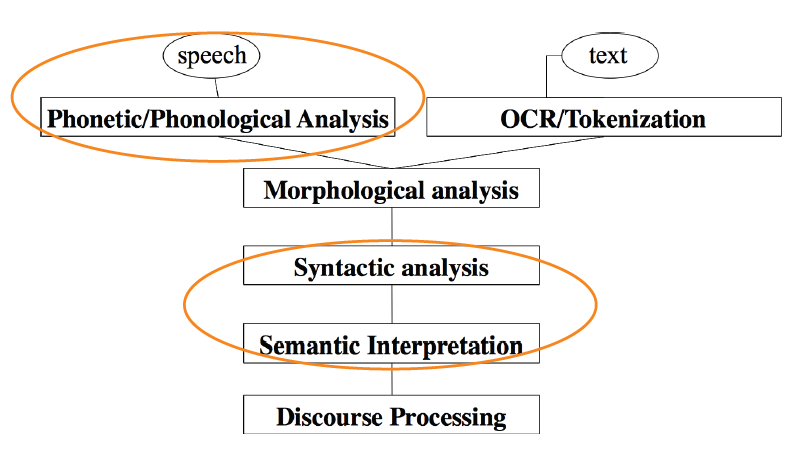
\includegraphics[scale=0.3]{nlp_level}
\caption{NLP Level}
\end{figure}

从图中可以看出,最基本的层次分为语音分析和文本OCR、切分,之后是语态分析(分析某些元素所祈祷的作用),之后是句法分析(对句子中的词语语法功能进行分析),再下一层是语义解释(分析每个成分在语义含义层面的事情),最后是语篇分析(所谓的终极理解)。各个问题都是研究的NLP的核心问题,难度和挑战也是逐层加大。
虽然NLP离完全AI还有很大距离,但当前的技术水平,以使它在各行业有了广泛的应用。

% 列表
\begin{itemize}
\item 拼写检查、关键词搜索、同义词查找
\item 信息提取,如提取价格、日期、地点
\item 文本分类、情感分析
\item 机器翻译
\item 对话系统,问答
\end{itemize}
在工业届很多实际场景中也得到广泛的应用。
% 列表
\begin{itemize}
\item 搜索场景(语音和文字)
\item 在线广告
\item 自动、辅助翻译
\item 市场情感分析
\item 语音辨识
\item 聊天对话系统(客服助手、设备控制、购物)
\end{itemize}

%1.2
\subsection{What's so special about human(nature) language?}
人类语言后者称作自然语言被设计的初衷是用来携带、传达彼此之间的信息,并不是由任何物理形成产生的,基于这一个特点,它不同于视觉、图像处理或其他机器学习任务。
举个具体的例子"rocket",这个词可以指代火箭这个概念,同时也可以表示具体事物火箭。不同的说话语气也可以表示不同的含义,比"Whooompaa".自然语言可以用多种形式进行表示,比如声音、手势、书写,这些信息不断的通过信号传送到人的大脑中,这样人才能去理解。
NLP的目标是通过设计算法让计算机能够理解自然语言并帮助执行一些任务。根据任务难度不同,NLP研究任务举例如下。

%列表
\textbf{Easy}
\begin{itemize}
\item 拼写检查
\item 关键词搜索
\item 同义词查找
\end{itemize}

\textbf{Medium}
\begin{itemize}
\item 文档解析
\end{itemize}

\textbf{Hard}
\begin{itemize}
\item 机器翻译
\item 语义分析(分析某个query的具体具体含义)
\item 指代分析(分析一篇文档中指称代词具体指的什么)
\item 问答系统
\item 聊天机器人
\end{itemize}
那么为什么要引入深度学习呢?因为深度学习可以看成是一个强大的表示学习系统,利用学到的representation去解决NLP相关的任务。现在问题来了,如和去得到一个词的表示,这个表示以何种形式进行存在呢?经过前人的探索和研究,将"word"表示成vector形式能够极大的促进任务的解决,因为word都以向量的形式进行表示,则可以进行距离方式(Jaccard, Cosine, Euclidean)进行计算。

% 2节
\section{Word Vector}
将word表示成vector对解决NLP Task有着重要的帮助,如何将word转换为vector呢?最直观的想法是建立一个vocabulary,然后将每个word都表示成一个vocab 大小的vector,vector中只有在word出现的index位置为1,其他位置全部为0,这种方式就是常说的基于BOW(bag of words)的\textbf{one-hot}编码。这种方式的缺陷显而易见,一是vocabulary词典很大,英文词典可达到13million,而中文词典更大;二是这种方式并不能体现同义词之间的相近关系。根据one-hot encoding的结果,计算任意两个词间的点积,结果都是零,这就是体现了这种encoding方式并不能体现出词间的某种相似性。除one-hot encoding之外,还有字符编码等。
% 图片2
%\begin{figure}[!htb]
%\centering
%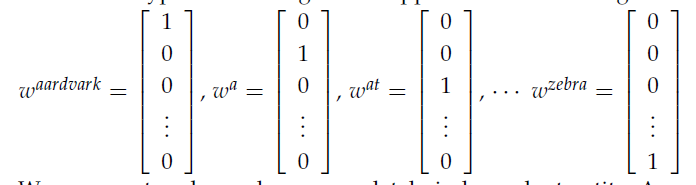
\includegraphics[scale=0.3]{one_hot_encoding}
%\caption{One-hot encoding}
%\end{figure}

% 3 节
\section{SVD Based Methods}
除了前面提到的one-hot encoding之外还可以利用基于矩阵分解对的方式来获得word vecotr(通常也称作word embedding)。这种方式有个前提假设,“经常同时出现的词语义具有相似性,即词间的共现性。” 首先我们遍历一个大的document库,目的是要构建一个word-document 矩阵。首先构建个vocabulary,然后遍历每个word \emph{i}在每个document \emph{j}中出现的次数,存放在$X_{ij}$,这样就形成了一个矩阵$X_{\emph{R}\emph{M}}$,M是总的文档数量。
当构造出word-doc矩阵之后,利用SVD(Singular Value Decomposition)对矩阵进行分析,矩阵分解公式如下,
%公式自动编号,
\begin{equation}
X = \emph{US$V^T$}
\end{equation}
进行矩阵分解之后,观察奇异值(对角矩阵S中对角线上的值),然后选取k个值,从而选择子矩阵$U_{1:V, 1:k}$ 作为word embedding 矩阵,那么每个词将表示成一个k-dimension的vector。这中方式其实类似于\textbf{LSA}。但同时这种方式也存在一些问题,如下:

% 列表
\begin{itemize}
\item word-doc矩阵经常变换,因为频繁会有新的词加入进来
\item 整个矩阵会非常系数,因为有很多词并不共现
\item 矩阵维度很大
\item SVD复杂度是O($n^2$)
\item 对于词频率不均衡需(有些词频率会很大)要特殊处理
\end{itemize}


% 4节
\section{Iteration Based Methods - Word2Vec}
换一种思维,设计一种模型,让模型的参数词向量,通过对模型的迭代训练、误差优化、参数更新学到word vectors。在NLP任务中,学者们已尝试过很多中方式来实现这个目的。比如在特定的NLP任务中,刚开始时将每个word转换为一个词向量,训练不仅仅更新模型参数同时也训练word vector。(注:这在tensorflow中是基于look table实现)。这里介绍一种更高效、简单的、概率的方法\textbf{word2vec},它是一个软件包,包含两种算法 \textbf{CBOW}(continuous bag-of-words)和\textbf{Skip-gram}。前者是给定context word 来预测center word,后者刚好相反;两种训练方法\textbf{Negative Sampling} 和\textbf{Hierarchical Softmax},负采样通过负采样来定义目标函数,分层softmax通过一种高效的树结构计算词典中每个词概率来定义目标函数。下文会对他们进行详细阐述。

% 4.1
\subsection{Continuous Bag of Words Model(CBOW)}
给定context word(上下文周边词)来预测center word的方式被称作CBOW模型。CBOW网络结构如图所示。
% 图
\begin{figure}[!htb]
\centering
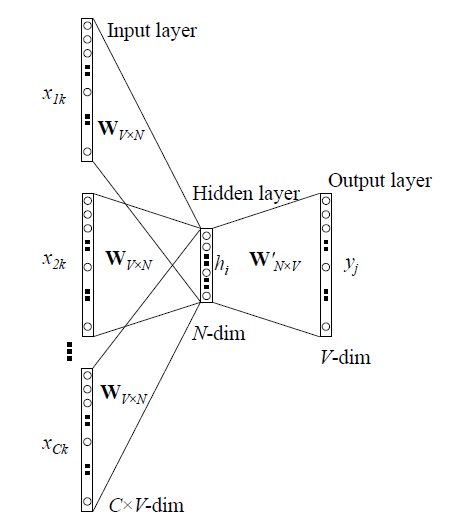
\includegraphics[scale=0.8]{cbow}
\caption{Continuous bag of words model}
\end{figure}

下面给出模型中一些必要的参数定义和说明:
% 列表
\begin{itemize}
\item $\textbf{\emph{V}}\in{n \times |{V}|}$, 输入词矩阵;n是词向量的embedding size即词向量的维度,|V|是vocabulary的大小,每一列\emph{$v_{i}$}表示$w_{i}$的词向量,维度为$n \times 1$,矩阵中每个元素值是通过模型训练得到。
\item $\textbf{\emph{U}} \in{|V| \times n}$, 输出词矩阵;n、|V|含义同上;每一行\emph{$u_{j}$}表示输出词\emph{$w_j$}的词向量,维度为$n \times 1$
\item \emph{c}代表中心词的下标
\item \emph{m}代表词窗口大小,即中心词前后几个词
\end{itemize}
在CBOW中每个词会学习到两个vector,输入词向量$v_i$和输出词向量$u_j$,最终选择哪个作为后文会讨论。CBOW模型执行具体过程如下.
% 列表
\begin{enumerate}
\item 对给定窗口大小m中的词进行one-hot编码,$(x^{(c-m)},...,x^{(c-1)},x^{(c+1)},...,x^{(c+m)}\in R^{|V|})$
\item 通过与输入词矩阵\textbf{\emph{V}}相乘得到词的embedded vectors,$(v_{c-m}=\emph{V}x^{(c-m)}, v_{c-m+1}=Vx^{(c-m+1)},...,v_{c+m}=Vx^{(c+m)} \in R^{n})$
\item 计算context vector的平均值,$\widehat{v}=\frac{v_{c-m}+v_{c-m+1}+...+v_{c+m}}{2m} \in R^{n}$
\item 计算vector score $z=U\widehat{v} \in R^{|V|}$,对于两个向量来说,距离越近点积越高,所以为了能够得到较高的分数,这个过程会将两个向量推向更加靠近。
\item 利用softmax进行概率化,$\widehat{y}=softmax{z} \in R^{|V|}$,softmax形式为$p_{i}=\frac{e^{u_i}}{\sum_{j}{}e^{u_j}}$,为什么采用指数形式,目的是转换为大于0的值,分母用来做归一化,是的所有值累计和为1。
\item 我们的目的是希望生成的概率值$\widehat{y} \in R^{|V|}$尽可能的接近真实的概率$y \in R^{|V|}$(one-hot编码而成)
\item 计算loss,这里由于是比较两个概率分布之间的差异,所以我们选择cross entropy $H(\widehat{y}, y)= - \sum_{j=1}^{|V|}y_{j}log(\widehat{y}_{j})$
\item 计算梯度,更新矩阵\textbf{V}和\textbf{U}
\end{enumerate}

以上就是CBOW模型具体执行过程,其中省略了梯度推导和计算.



% 4.2
\subsection{Skip-gram}
Skip-gram是通过中心词来预测周围词的模型。skip-gram网络模型如图所示。
% 图
\begin{figure}[!htb]
\centering
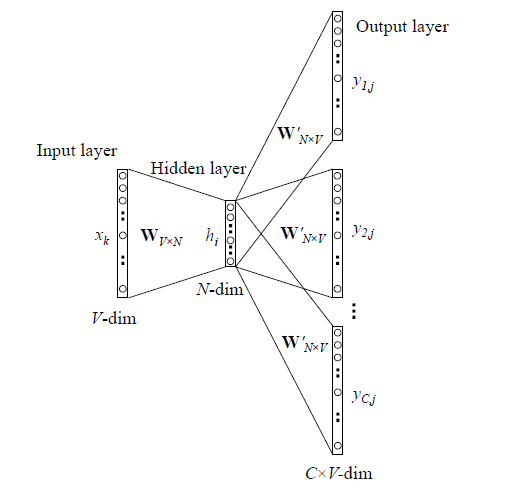
\includegraphics[scale=0.3]{skip-gram}
\caption{Skip gram model}
\end{figure}
skip-gram 模型过程基本与CBOW类似,下面对该过程进行具体介绍。
% 列表
\begin{enumerate}
\item 生成中心词的one-hot词向量$x \in R^{|V|}$作为输入
\item 得到中心词的embedded 向量 $v_{c}=Vx \in R^{n}$, V是输入词矩阵与CBOW含义相同
\item 就是vector score $z=Uv_{c} \in R^{|V|}$, 这里得到的是中心词 m窗口附近的词
\item 概率化,$\widehat{y}=softmax{z} \in R^{|V|}$,这里预测值是$(y_{c-m},...,y_{c-1},...,y_{c+m})$,真实值是one-hot向量
\item 计算损失,这里有个重要假设(Naive Bayes Assumption),给定输入中心词,所有输出词是独立的。因此可以直接利用cross entropy计算误差
\item 计算梯度,更新参数和向量
\end{enumerate}

在CBOW 和Skip gram 模型中,采用的方式是用生成的一种概率分布去预测词的真实分布,如何去评价模型的好坏呢?根据信息论我们知道,cross entropy是用来测度两个分布之间差异,因此在CBOW和SG模型中也采用交叉熵作为目标函数。在SG模型中,基于朴素贝叶斯假设,将预测的上下文词的联合概率分布当做独立分布去计算。这里以SG模型为主,且词窗口设定为1,则目标函数为
$$J = H = -y_{i}log(\widehat{y_{i}}) = -log(p(u_{c}|v_c)) = -log\frac{exp(u_{c}^{T}v_{c})}{\sum_{w=1}^{|V|}exp(u_{w}^{T}v_{c})}$$
其中,$y_i$是真是词向量,属于one-hot编码只有在下标为c处为1,而预测概率$\widehat{y}$是通过softmax而来。以上就是最终的目标函数,可以基于此目标函数对其中的输入参$v_{c}$和输出参数$u_{c}$就梯度,采用梯度下降法进行求解最优值。
\textbf{TODO,梯度过程推导}各参数梯度求导可参考文献\href{http://shomy.top/2017/07/28/word2vec-all/}{[1]}


% 4.3 
\subsection{Negative Sampling}

% 4.4
\subsection{Hierarchical Softmax}





\end{document}